
\section{Simulation and Results}
\label{sec:simulation}

In this section we will test the proposed \disr{} approach to
demonstrate its effectiveness and compare it against a topology
agnostic approach based on spanning trees and
broadcasting~\cite{Patwardhan05evaluatingthe}, to measure how \disr{}
performs in covering the network structure. Note that a direct
comparison against the SR segment-based approach is not addressed
here, since how described in Section~\ref{sec:introduction} our
scenario assumes the non-feasibility of a centralized approach:
however, all the properties of the centralized approach should be
considered as preserved for all the nodes reached by the distributed
segment coverage of \disr{}. Thus, the main points that remain to be
addressed are:
\begin{itemize}
\item how \disr{} compares against state-of-art of tree based approach
applied to equivalent scenario
\item how \disr{} scales on large networks
\item the real feasibility of the required hardware on the limited
node size assumed
\end{itemize}

%\item Against the centralized segment based approach (SR), to evaluate
%if and how its known properties are still preserved in the new nano-scale distributed scenario

\subsection{Nanoxim Environment}

In order to quantitatively and qualitatively evaluate the proposed approach a
specific simulation environment has been developed, resulting in
the open-source and freely available project called
Nanoxim~\cite{nanoxim}.
Nanoxim is a SystemC tool based on an almost rewritten
version of the Noxim Network-on-Chip simulator~\cite{noxim}. While some
complex features have been removed (e.g. wormhole, congestion/topology
aware routing and selection strategies) new features specifically
tailored for the nanoscale scenario were introduced, e.g. the ability to simulate a random
network, the implementation of \disr{} to obtain the segment topology
and the support for defective links and nodes.

%------------------------------------------------------------------------------
\subsection{Experimental setup}
The following parameters have been taken into account when
performing the \disr{} simulation:
\begin{itemize}
\item {\emph{Size of the network}}: number of nodes, on a range from
10x10 to 100x100 sized networks. 
%\item {\% defective links}: the probability that each link is
%disconnected or not present, from 0 the amount that yields
%no more segments.
\item {\emph{\% defective nodes}}: the probability that a node is not
working, thus having all its links not able to be utilized during \disr{} setup.  
%Same range as defective links parameter.
\item {\emph{Bootstrap node}}: the node from upper layer that
injects the \disr{} process. When not explicitly investigating the
impact of each single bootstrap choice, a set representative regions have been
considered, e.g. the central part of the network and the edge corners.
\end{itemize}
To present the results, the following evaluation metrics have been adopted:
\begin{itemize}
\item{\emph{Node coverage}}: this is the fraction of nodes that
are assigned to a segment. In the ideal case, all the non defective
nodes should be assigned, so this metric is useful to show how some
disconnected regions can negatively impact on the whole \disr{}
effectiveness.
\item{\emph{Latency}}: this measures how the cycles required to complete the
segment assignment scale for increasing network sizes and defect rates.
\item{\emph{Bootstrap node effect}}: this evaluates the impact of the chosen
bootstrap node on the node coverage.
\end{itemize}

%Further, to evaluate how \disr{} compares against the centralized segment
%based algorithm, the following metrics have been adopted:
%\begin{itemize}
%%\item {Average Path Length}:
%%\item {Average Link Weight}:
%\item {Unidirectional restrictions:}
%\item {Number of Segments}:
%\end{itemize}

Since the distribution of defects and thus the resulting topology is randomly
generated, a set of simulations with different seeds has been run
for each system configuration. We found that 20 repetitions are
required in order to obtain statistically significant results.


\subsection{Results}
\label{sec:results}

In this section we analyze the results in terms of node coverage and
latency with different network sizes, defect rates and bootstrap
injection points. In particular Figure~\ref{fig:results_coverage}
shows node coverage for \disr{} and Reverse Path Forwarding (RPF) tree
based approach (as adapted in \cite{patwardhan_nanoarch06}) respectively. While the first aim of \disr{} is not to
reach the optimal coverage, we still can observe a quite good
performance as compared to the tree based approach. For low defect
rates, i.e. below 10\%, both approaches reach near ideal coverage for
each of the tested network sizes. Higher defect rates seems to show
more variance for \disr{}. For example at the high 20\% rate \disr{}
ranges from 60\% to 75\% while RPF remains stable at 75\%. However we
can consider this coverage sensibility at higher defect rates as still acceptable
for this first, not yet optimized version of the proposed approach.
Note that defect rates beyond 25\% lead to many disconnected
regions of nodes that \disr{} currently cannot handle. This threshold can be
intuitively related to the fact that in the topologies simulated a
node has (on average) a cardinality of 4 connections to other nodes. This means
that with a defect rate bigger than 25\% a node has at least one of its four
paths as not-working, and this applies (on average) for each node,
thus leading to increased probability of consecutive disconnected
nodes, which eventually create disconnected regions. For example Figure~\ref{fig:net} shows a 30x30 network with a 25\%
defect rate in which the bottom-left part cannot be reached due to
disconnected regions. Note that the remaining defective nodes belonging to
connected regions are successfully surrounded by \disr{} coverage; in any
case, these defect levels should be considered as worst case scenarios, so the
achieved coverage of $0.5$ is a satisfying result for this first
version of \disr{}. On the other hand, the network size seems to have a
limited impact when defect rate does not introduce too many disconnected
regions. 
\begin{figure*}
\centering
\begin{tabular}{cc}
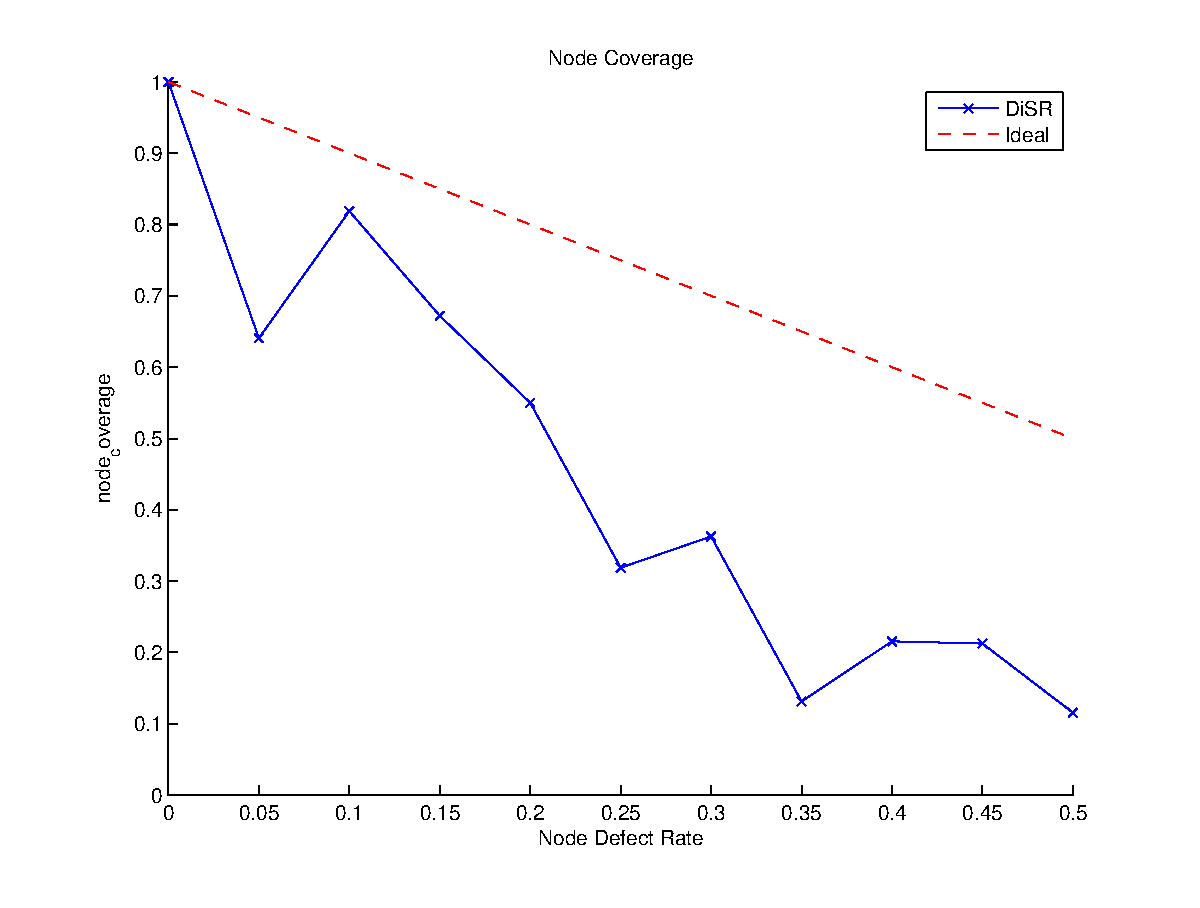
\includegraphics[width=0.48\textwidth]{pictures/set1.eps} & 
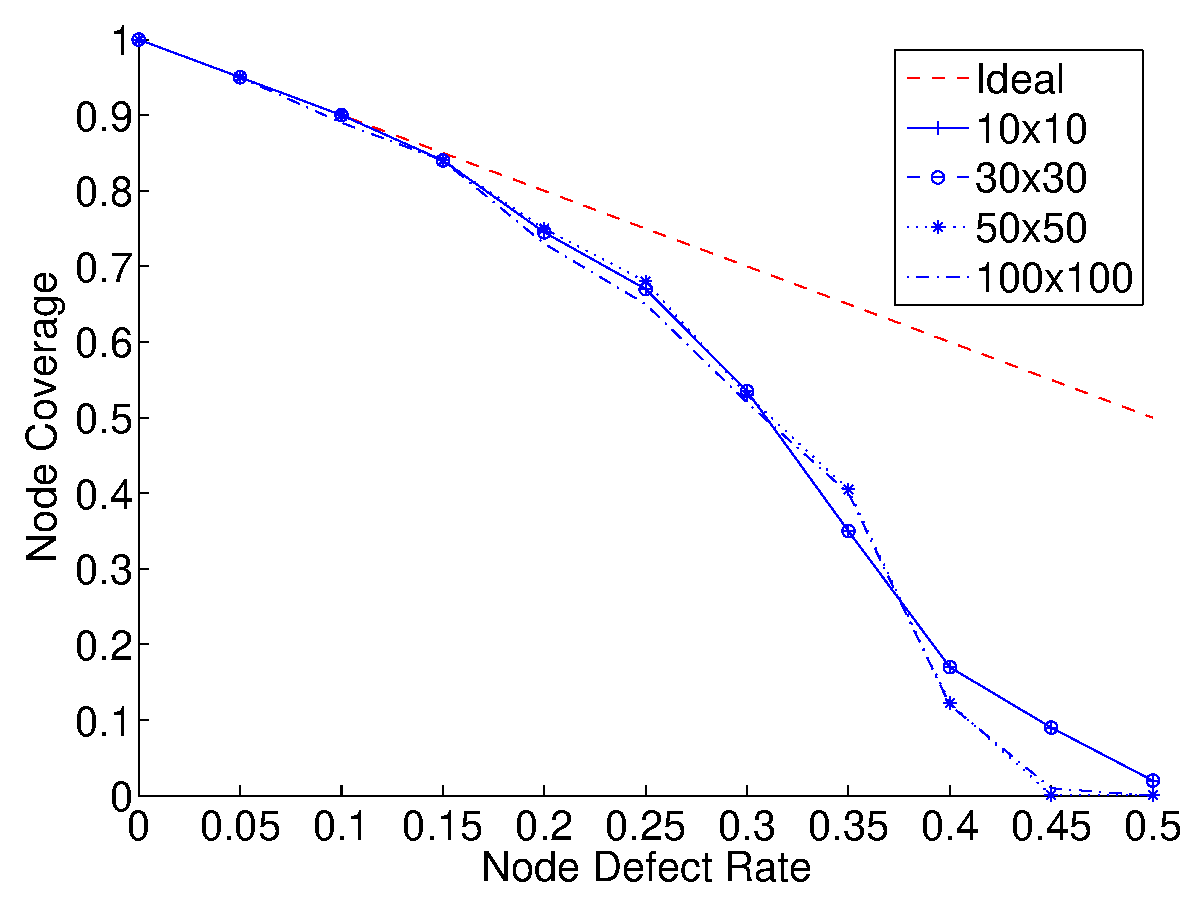
\includegraphics[width=0.48\textwidth]{pictures/coverage.eps} \\
(a) & (b) 
\end{tabular}
\caption{\disr{} (a) and RPF (b) node coverage}
\label{fig:results_coverage}
\end{figure*}

\begin{figure*}
\centering
\includegraphics[width=0.70\textwidth]{pictures/net.ps}
\caption{Covered regions in a 30x30 network with 25\% of defects}
\label{fig:net}
\end{figure*}

\begin{figure*}
\centering
\begin{tabular}{cc}
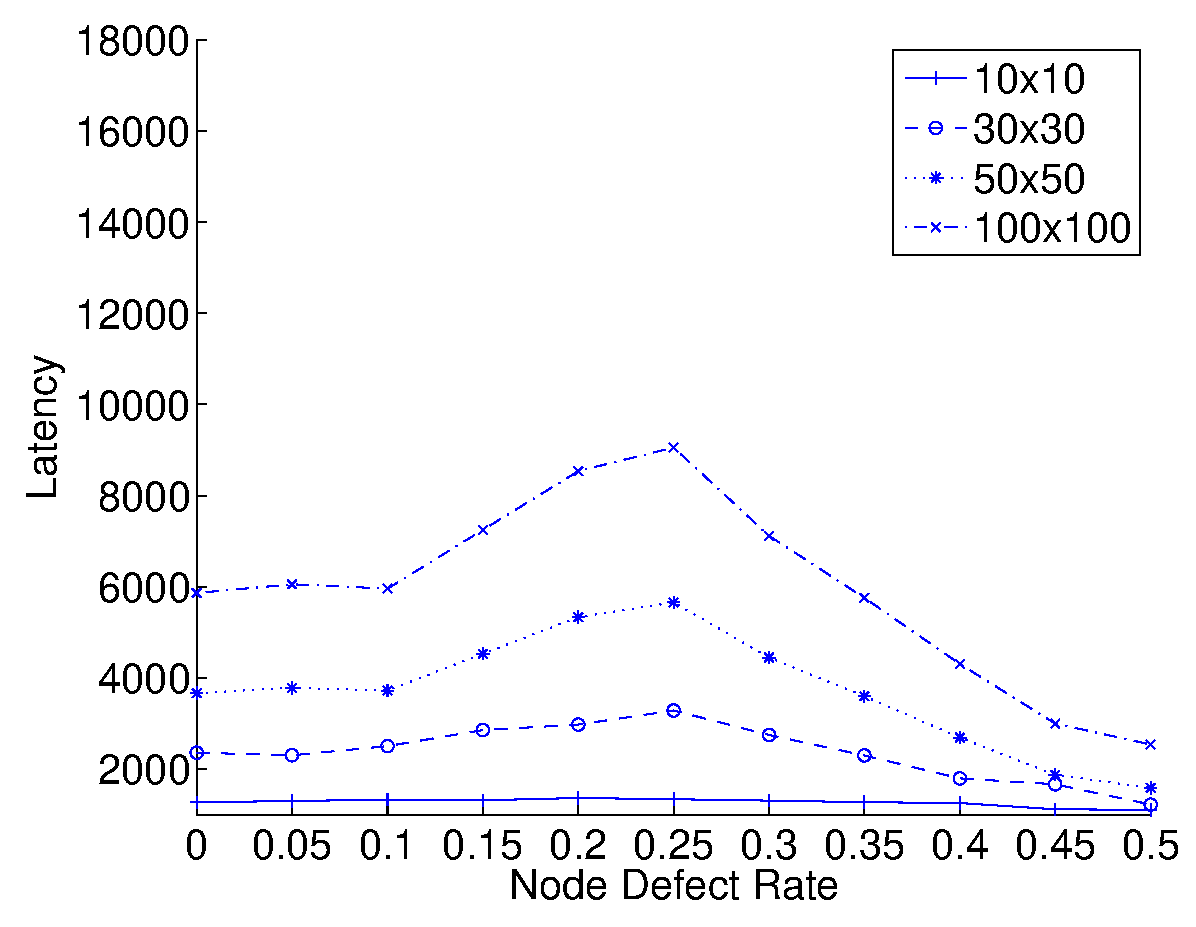
\includegraphics[width=0.48\textwidth]{pictures/set2.eps} & 
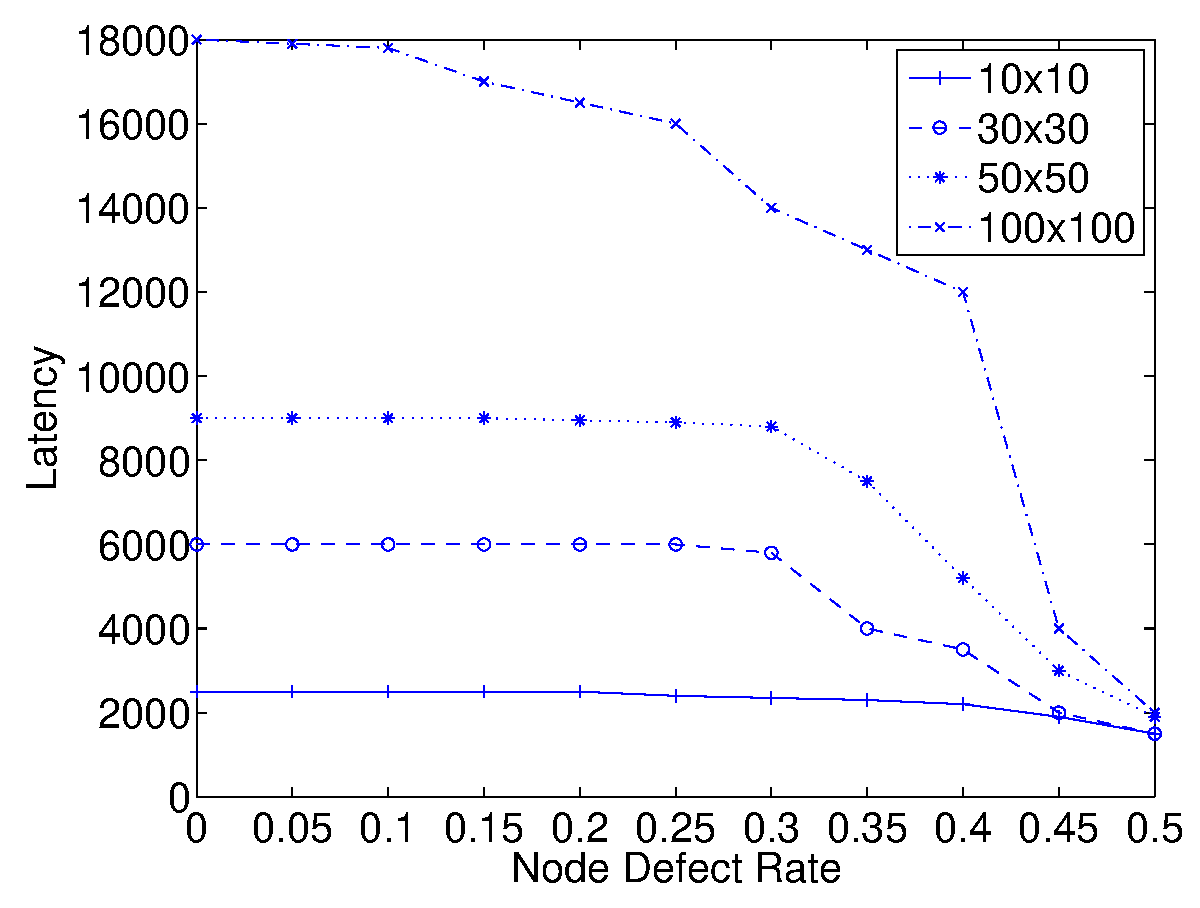
\includegraphics[width=0.48\textwidth]{pictures/set2_rpf.eps} \\
(a) & (b)
\end{tabular}
\caption{Latency of \disr{} (a) vs tree based RPF (b) }
\label{fig:results_latency}
\end{figure*}

The number of cycles required to complete segment mapping process is
shown in Figure~\ref{fig:results_latency}. In this case the comparison
against the tree-based approach shows better (lower) values at
different defect rates. Rather than the absolute numbers, what is more
interesting to observe is how \disr{} latency scales with network
size. For example, going from 900 to 2500 nodes, at the medium defect
rate of $0.15$, leads to an increase from 3000 to 4500 cycles. It
should be noticed also how for \disr{} latency is increasing until the
threshold of $0.25$ is reached, meaning that the completion of the
process is more and more difficult due to the missing paths, but
\disr{} is still able to finish the segment discovery using the retry/cancel mechanisms
described in the previous section. This initial behavior is not reported in
the RPF based approach, leading to higher latency values and not using
the same retry/cancel approach as \disr{}.

After the $0.25$ threshold, the impact of disconnected regions
becomes predominant and both approaches become faster in completing
the covering process, since far less nodes can be actually reached. 

Finally, Figure~\ref{fig:results_bootstrap} visually represents the
stability of the approach against a different bootstrap node choice
in a 10x10 network. This is an important aspect to evaluate 
considering that one of the main advantages of \disr{} against all the
tree-based approaches is the possibility of choosing whatever
bootstrap node, without having to care about the role assumed in the
future by the chosen root node. In other words, after the segments have
been established, the bootstrap node is like every other node, i.e. it
is not center of a structure, and it is not an hotspot for the traffic
distribution. The results in terms of coverage, shown for low, medium
and high defect profiles, demonstrate a relatively limited
impact of the bootstrap node choice in the low/medium scenarios, while a
$30\%$ instability is found for very high defect rates. This also
sounds acceptable, since when a lot of defective nodes are present, the
particular position of the bootstrap node could lead to a completely
different evolution in the \disr{} setup process.

\begin{figure}
\centering
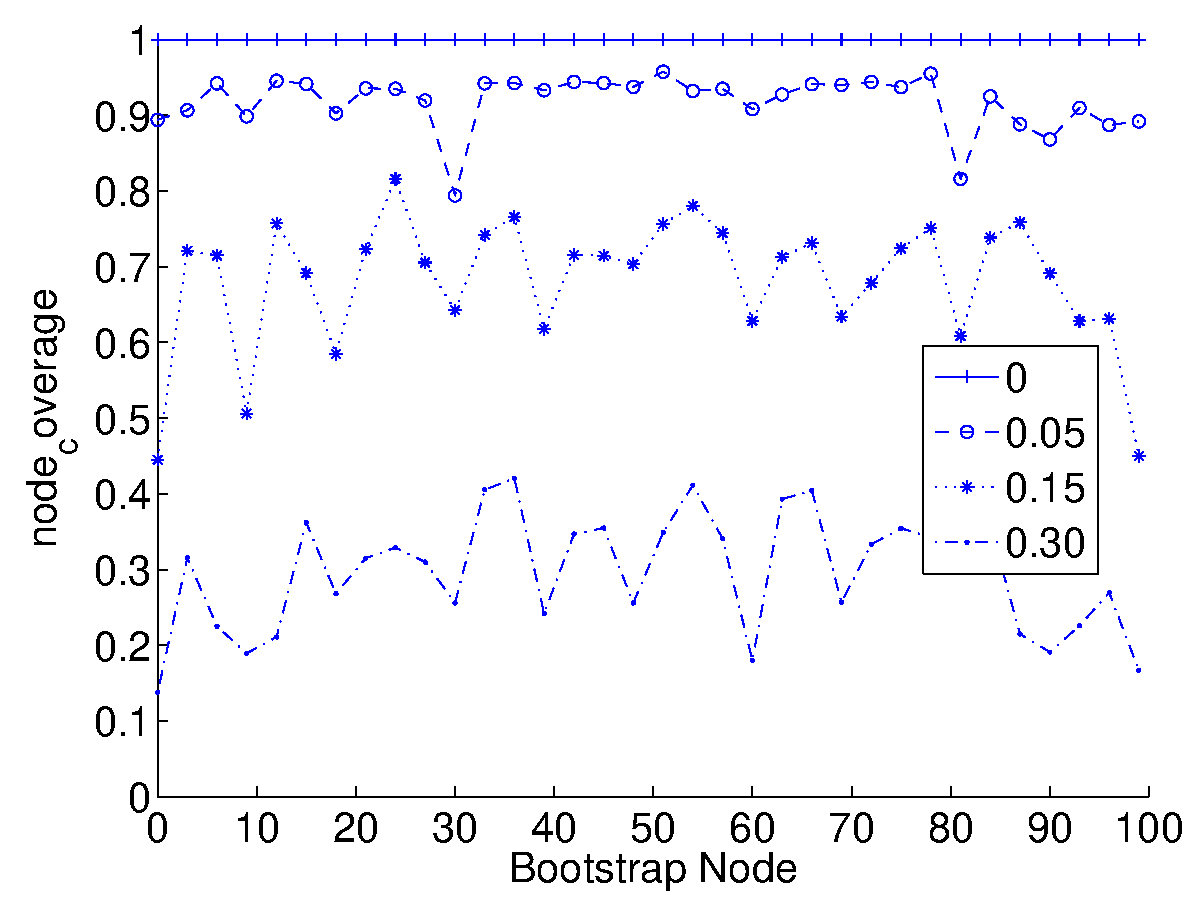
\includegraphics[width=0.48\textwidth]{pictures/set3.eps}
\caption{Effect of bootstrap node}
\label{fig:results_bootstrap}
\end{figure}

% TODO: long paper
\subsection{Other Optimizations}
Some optimization parameters, which demonstrated to improve the \disr{}
results, have been fixed to some reasonable default values (see below) and are not subject to
further investigation in this paper; once again the focus here is not the
optimal setup of segments, but just demonstrating a working approach. 
These parameters are:
\begin{itemize}
\item \emph{cycle\_links}: max number of retries across the set of links of
each node. While searching for a free link due to an incoming \texttt{SEGMENT\_REQUEST},
the request itself is cancelled after a given number of tries. This
gives to the preceding node on the path the
chance to test a different route instead of waiting indefinitely.
Default value is set to 1, i.e. each link is tried one time.
\item \emph{time to live (TTL)}: when a segment request is cancelled
along a certain path (using a \texttt{SEGMENT\_CANCEL}), a TTL field is
decreased in the request packet, so that requests that have been
denied too much times can desist, even if free links are
available. This is not only an optimization to shorten
requests' processes, but also solves some critical situations in which
request packets are blocked in routing loops in a particular path.
\item \emph{bootstrap\_timeout}: number of time units that a bootstrap node
should wait before assuming that a livelock in the starting segment
process has occurred. In the worst case, we can imagine that longest
path required is the one returning to the bootstrap node after having
traveled across all the links. So, although this is just an extreme
situation, a good upper limit can be safely be set to $N \times N$.
\item \emph{bootstrap\_immunity}: in order to avoid the failure of the whole \disr{}
setup process, a bootstrap node should not have defective links.
Enabling this optimization, a bootstrap node is immune to defects.
We may think about a pre-bootstrap phase that properly selects (from upper
layer via) a bootstrap node which is tested as properly connected. We
enabled this optimization, however empirical tests have shown us that only
simulations using bootstrap nodes placed on edges would be heavily
affected by similar issues since these nodes start with a lower number of links,
e.g. corner nodes could only have two connected direction, so even a single
defective link could prevent a starting segment packet from coming back to the
bootstrap node to close the loop and create the first segment.
\end{itemize}
